\section{Teilversuch 4: Betrachten des Auf- und Entladevorgangs eines Kondesators}
	Die Kurve von \texttt{[CHI]} ändert sich während des gesamten Teilversuchs nicht. Das ist auch erwartet, da die Ausgangspannung des Frequenzgenerators unabhängig von der Schaltkreis sein soll. 
	\begin{multicols}{2}
		\begin{figure}[H]
			\centering
			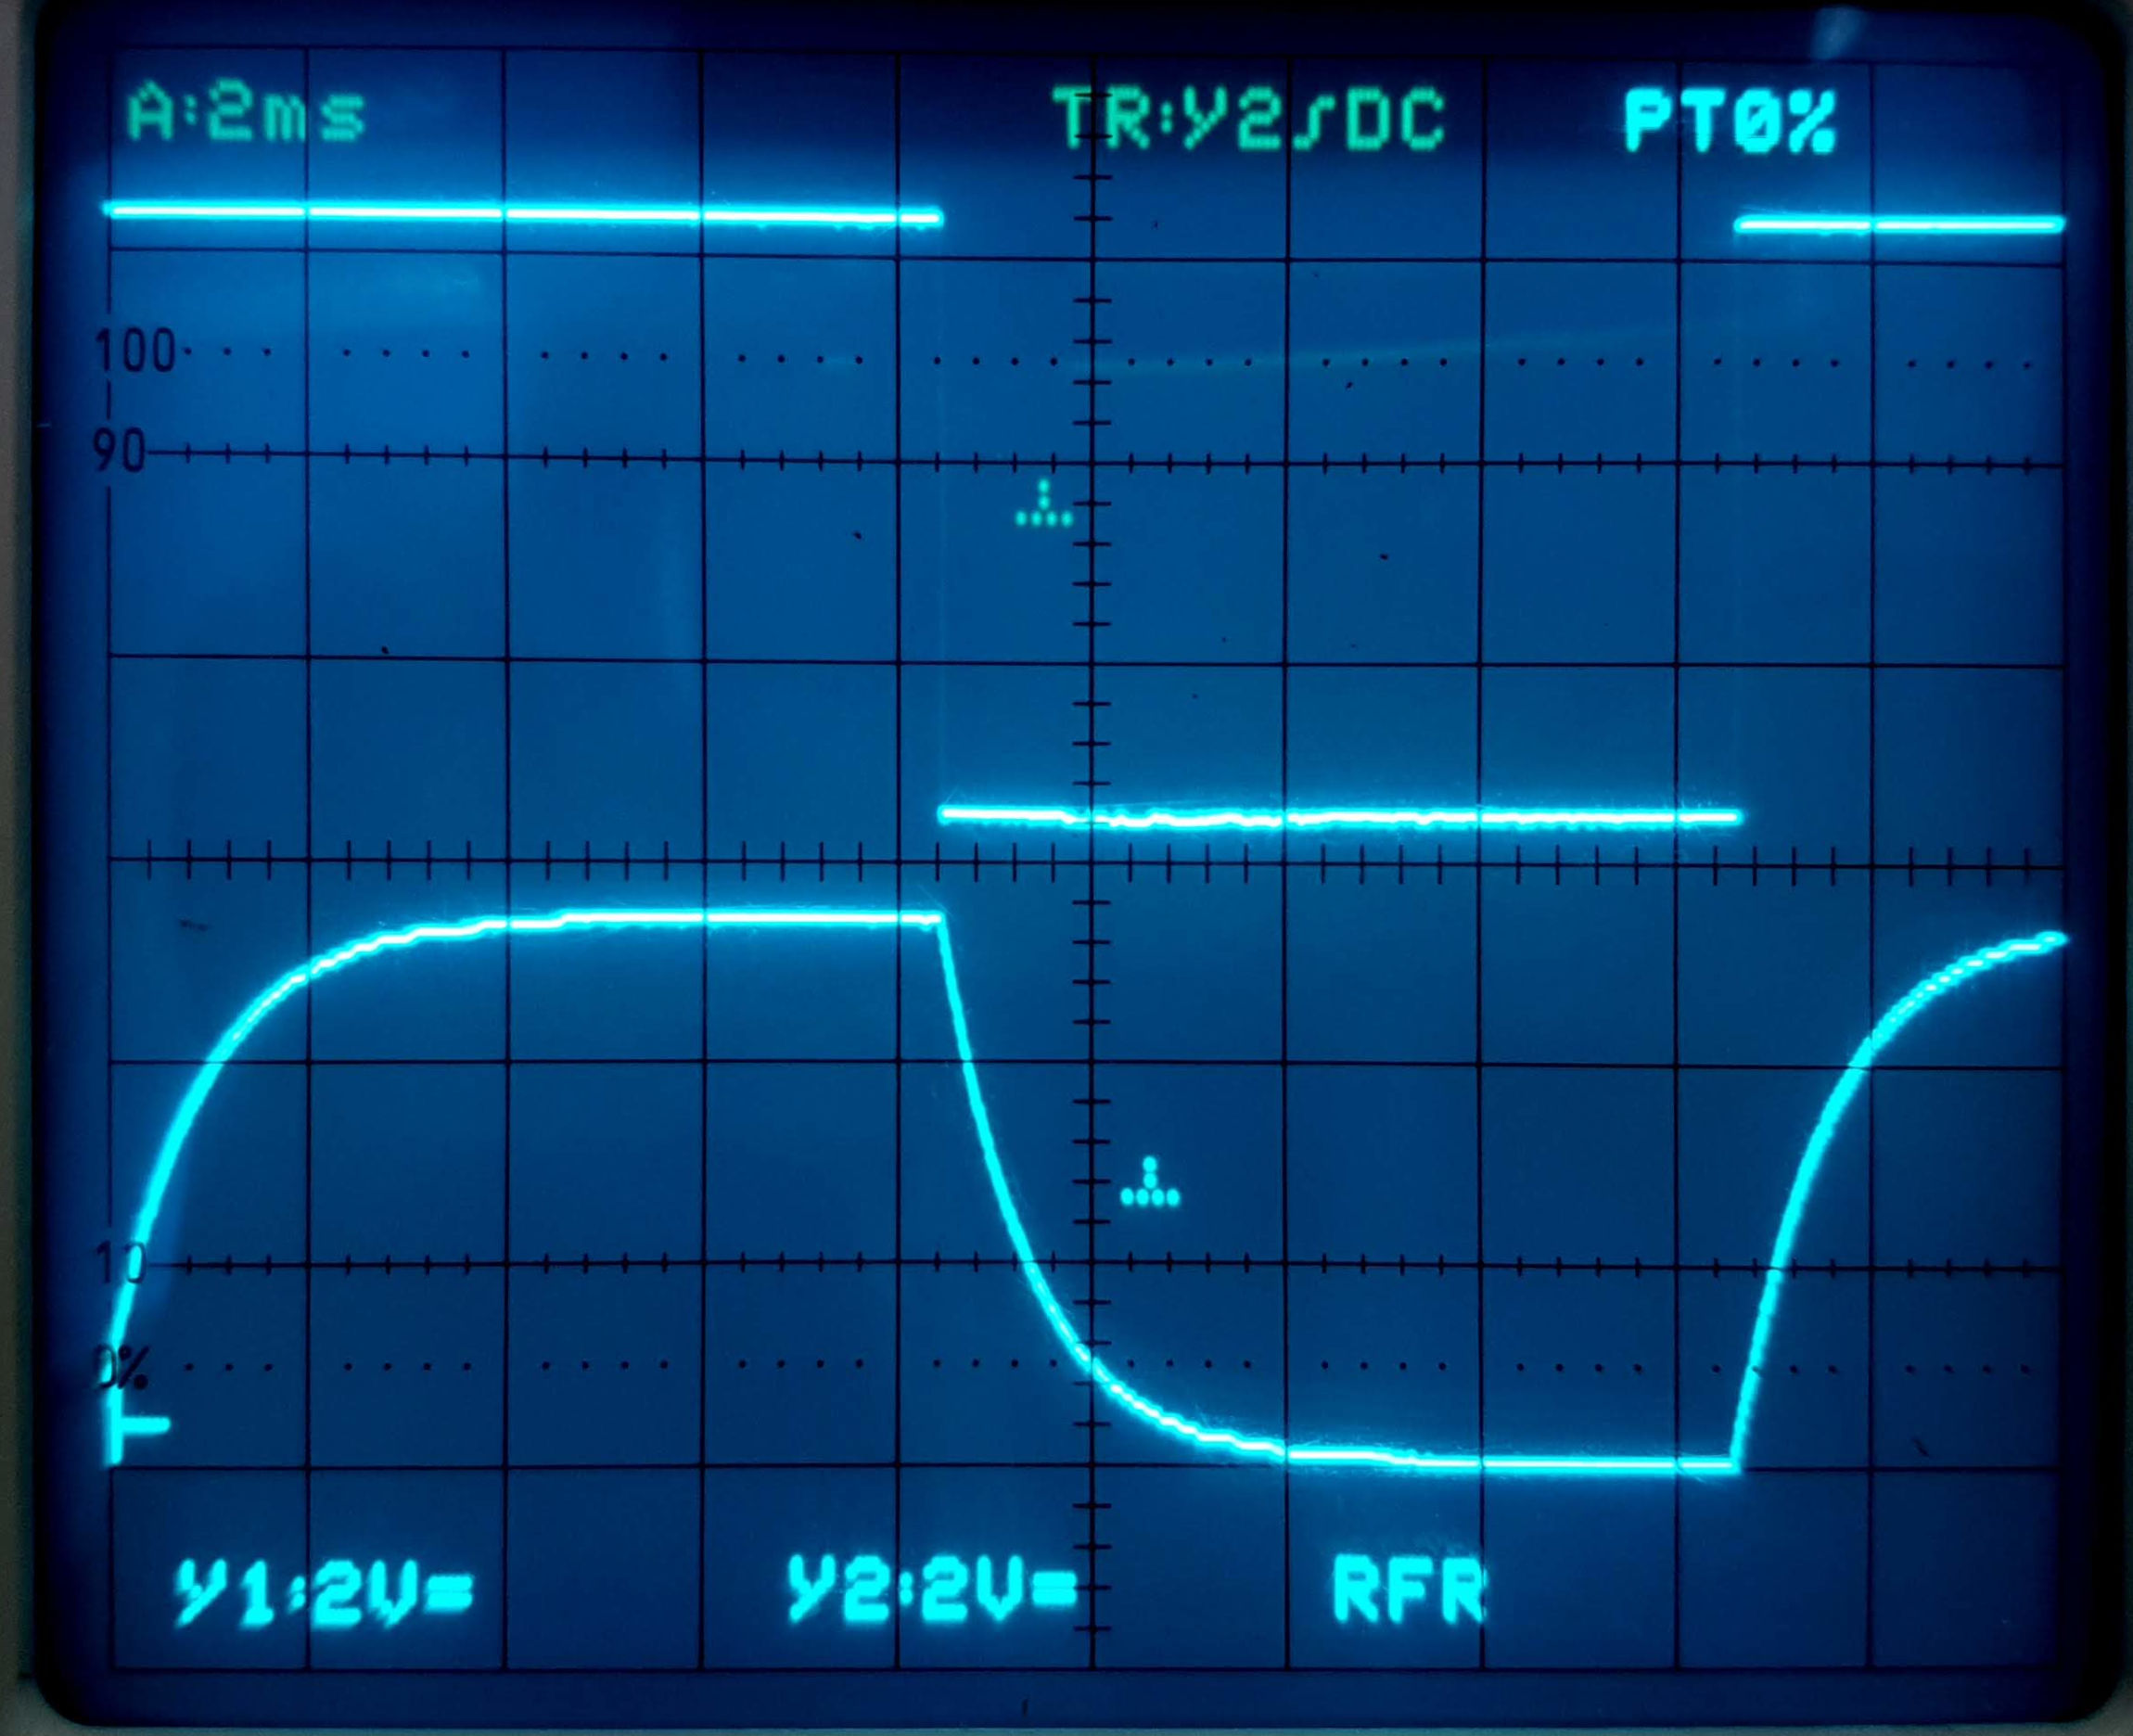
\includegraphics[width=0.4\textwidth]{images/low-widerstand.jpg}
			\caption{\centering Kleinerer Widerstand}
			\label{fig:low-widerstand}
			\vspace{-1em}
		\end{figure}
		\begin{figure}[H]
			\centering
			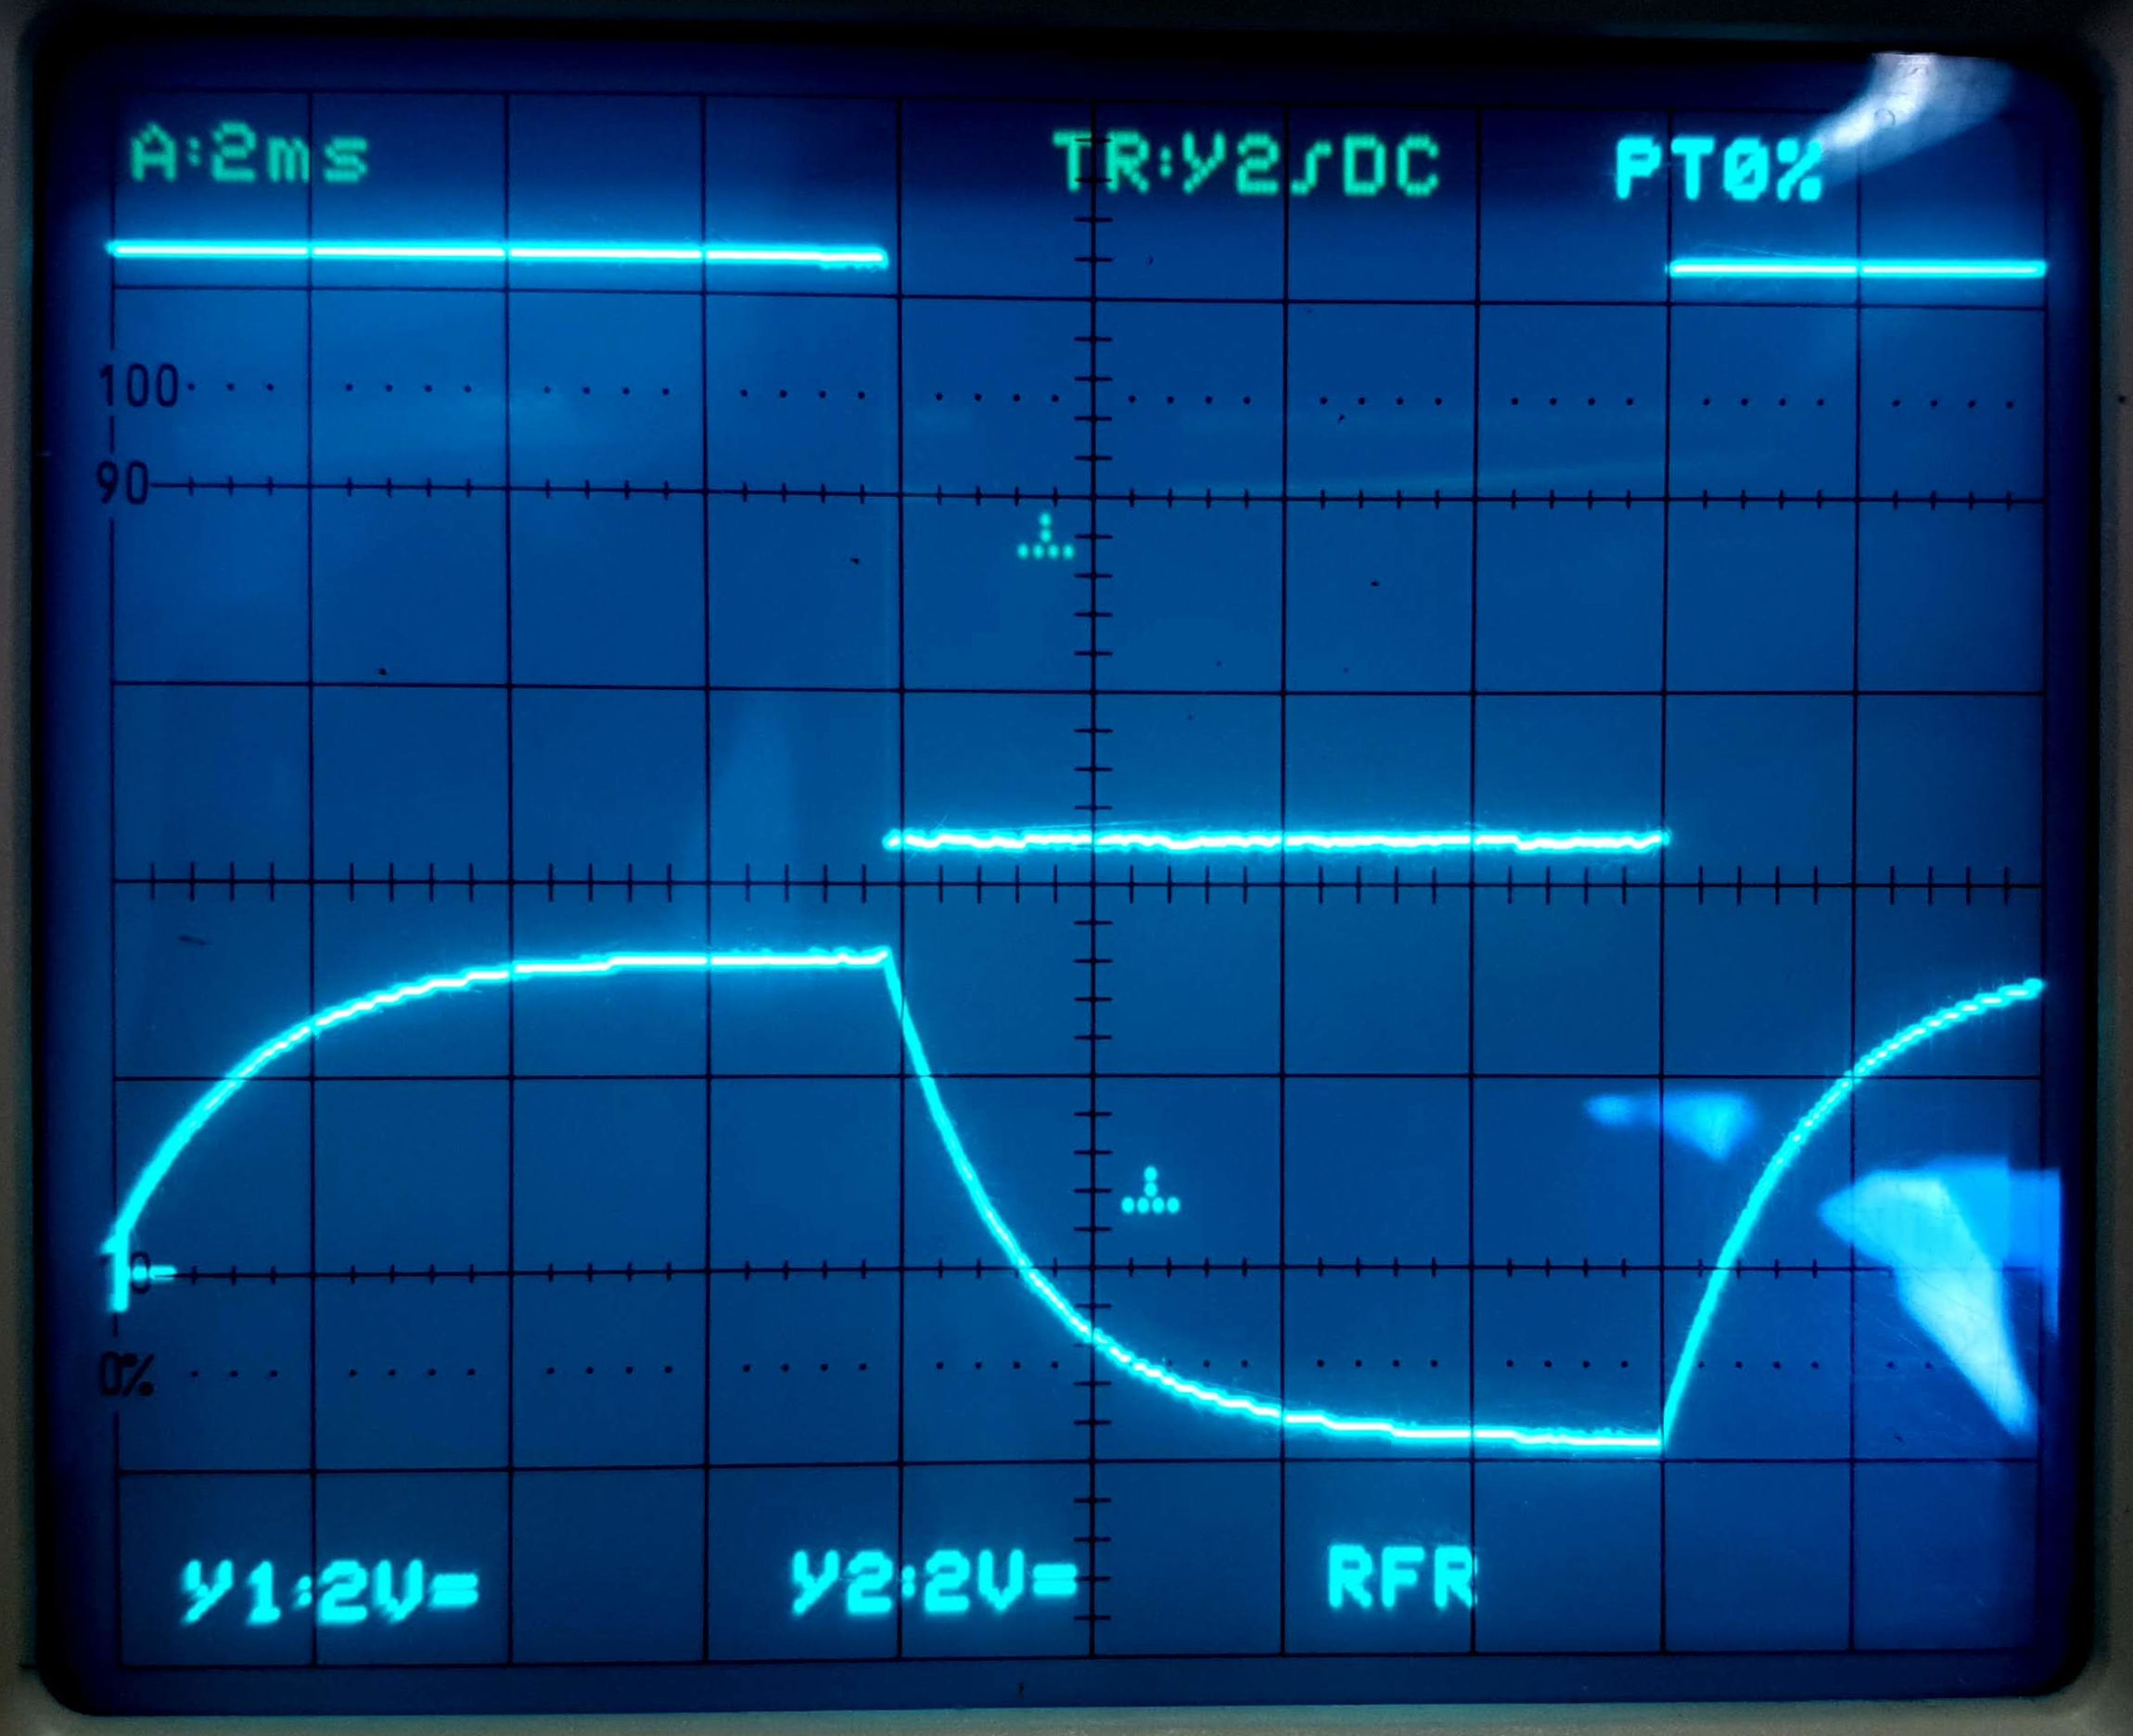
\includegraphics[width=0.4\textwidth]{images/high-widerstand.jpg}
			\caption{\centering Höherer Widerstand}
			\label{fig:high-widerstand}
			\vspace{-1em}
		\end{figure}
	\end{multicols}
	Mit zunehmendem Widerstand wurde die Kurve flacher. Intuitiv erfahren die Ladungen mehr Widerstand, wenn sie aus dem Kondensator entlädt wurden. Es braucht deswegen mehr Zeit, um der Kondesator komplett zu entladen, was die Kurve flacher macht. Mit dem zweiten Kondesator im parallel zum Ersten ist die Kurve auch flacher. 

	Aus der Theorie gilt:
	\begin{align}
	 	U_C = U_0 \exp\left(-\frac{t}{RC} \right) && \text{bzw.} && t_e = RC
	\end{align} 
	wobei $t_c$ die Relaxationszeit ist, was ein Maßstab dafür ist, wie schnell der Vorgang verläuft. 

	Im Experiment ist der Widerstand durch das Drehen am Potentialmeter erhöht. Mit dem anderen Kondensator parallel zum Ersten, erhöht man die Kapazität. Somit sind $R$ bzw. $C$ jeweils größer. Mit zunehmendem Widerstand $R$ bzw. Kapazität $C$, wird die Relaxationzeit länger, was hier beobachtet ist.